


%how to cite
%\cite{Seow2011}
%how to add figure



\newpage
\section{Introducci\'on}
\textit{Person in Charge; }

\subsection{s}
For governments and manufacturing companies, global warming, rising energy prices, and customers increasing ecological awareness have pushed energy efficient manufacturing to the top of the agenda. The integrating energy efficiency performance in production management, gap analysis between industrial needs and scientific literature. Manufacturing companies need greater capabilities to respond more quicker \cite{Ghani2012} to market dynamics and varying demands. It is obvious that energy efficiency becomes a driver for manufacturing industry, since it has become one of the greatest energy consumers and carbon emitters in the World, higher than transportation, residential and commercial usage. Like shown in Figure \ref{fig:TotalConsumption} 

\begin{figure}[h!]
	\centering
	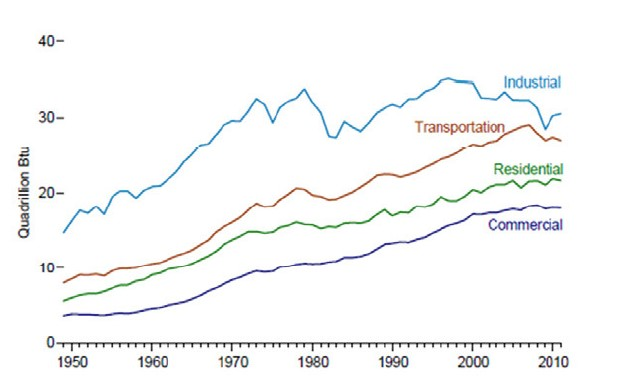
\includegraphics[width=0.8\linewidth]{Figure/Total-consumption.jpg}
	\caption{Total Consumption by End-Use Sector, 1949-2011 \cite{Apostolos2013}}
	\label{fig:TotalConsumption}
\end{figure}


